%% Seção 4: O Estado Emocional é Acumulado ao Longo do Tempo, Formando um Mapa Afetivo

\chapter{O Estado Emocional é Acumulado ao Longo do Tempo, Formando um Mapa Afetivo}

\epigrafe{O inconsciente é estruturado como uma linguagem.}{Jacques Lacan}

\textbf{4.} O estado emocional é acumulado ao longo do tempo, formando um mapa afetivo que pode ser compreendido e interpretado através da linguagem, permitindo a construção do self e a autonomia do ser.

\section{O mapa das emoções através da integral de expressões}

\textbf{4.1} A linguagem permite que o terapeuta trace um mapa das emoções através da integral de suas expressões discursivas, revelando padrões afetivos.

\begin{tese}
Se o estado emocional se acumula ao longo do tempo, então a linguagem pode ser utilizada para mapear e compreender esse acúmulo, formando um mapa afetivo.
\end{tese}

\begin{hipotese}[title=Hipótese 4.1.1 (Condicional)]
Se analisamos a linguagem do paciente ao longo do tempo, então podemos identificar padrões emocionais e mapear seu estado afetivo.
\end{hipotese}

\begin{referencia}[title=Referência a Lacan]
Para Lacan, a linguagem é estruturante do inconsciente; os significantes repetidos ao longo do discurso revelam as estruturas afetivas subjacentes.
\end{referencia}

\begin{aforismo}
Nas palavras que se repetem, o coração desenha seu mapa oculto.
\end{aforismo}

\section{Mapeamento emocional e soma das emoções}

\textbf{4.11} O mapeamento emocional é a soma das emoções expressas em função do tempo, permitindo a identificação de padrões e trajetórias afetivas.

\begin{tese}
Se o estado emocional pode ser representado como uma função ao longo do tempo, então a integral das expressões emocionais na linguagem fornece uma representação acumulada do estado afetivo.
\end{tese}

\begin{referencia}[title=Referência a Dennett]
A consciência pode ser vista como uma narrativa contínua; assim, o acúmulo de emoções na linguagem forma um fluxo narrativo que representa o self.
\end{referencia}

\begin{aforismo}
A soma das emoções contadas é a história que a alma narra a si mesma.
\end{aforismo}

%% Representação Matemática do Mapa Afetivo
\subsection*{Formalização Matemática: O Mapa Afetivo}

O estado emocional acumulado ($E_A$) pode ser representado como a integral das expressões emocionais na linguagem ($L_E$) ao longo do tempo:

\begin{equation}
E_A(t) = \int_{t_0}^{t} L_E(\tau) \, d\tau + E_0
\end{equation}

Onde:
\begin{itemize}
    \item $E_A(t)$ é o estado emocional acumulado no tempo $t$
    \item $L_E(\tau)$ é a expressão emocional na linguagem no tempo $\tau$
    \item $E_0$ é o estado emocional inicial
    \item $t_0$ é o tempo inicial
\end{itemize}

A taxa de mudança do estado emocional (derivada) seria:

\begin{equation}
\frac{dE_A}{dt} = L_E(t)
\end{equation}

Isto indica que a linguagem emocional atual determina a taxa de mudança do estado emocional acumulado.

\section{Mapa afetivo e padrões ocultos}

\textbf{4.12} Este mapa reflete as oscilações internas e revela padrões que, de outra forma, poderiam permanecer ocultos, auxiliando na compreensão profunda do self.

\begin{tese}
Se o mapa afetivo revela padrões emocionais ocultos, então ele é uma ferramenta valiosa para a compreensão e intervenção terapêutica.
\end{tese}

\begin{referencia}[title=Referência a Searle]
Os estados mentais possuem intencionalidade; compreender os padrões emocionais permite entender as intenções subjacentes e agir sobre elas.
\end{referencia}

\begin{aforismo}
Nos caminhos traçados pelo sentir, encontram-se as intenções que guiam o ser.
\end{aforismo}

\section{Análise longitudinal da linguagem}

\textbf{4.2} A análise longitudinal da linguagem permite ao terapeuta identificar as mudanças sutis no estado emocional do paciente, promovendo insights e autonomia.

\begin{tese}
Se a linguagem evolui ao longo do tempo, refletindo mudanças emocionais, então sua análise contínua permite identificar essas variações e promover a autocompreensão.
\end{tese}

\begin{referencia}[title=Referência a Guimarães Rosa]
A linguagem é viva e mutável; suas transformações refletem as mudanças internas do indivíduo.
\end{referencia}

\begin{aforismo}
A palavra que muda anuncia o vento que vira dentro da gente.
\end{aforismo}

\section{Progresso ou regressão do estado emocional}

\textbf{4.21} O progresso ou regressão do estado emocional pode ser expresso pela função derivada da linguagem ao longo do tempo, permitindo intervenções terapêuticas precisas.

\begin{tese}
Se a variação na linguagem reflete a taxa de mudança do estado emocional, então podemos utilizar essa informação para ajustar o processo terapêutico.
\end{tese}

\begin{referencia}[title=Referência a Wittgenstein]
A linguagem é uma forma de vida; suas mudanças refletem mudanças nas formas de vida do indivíduo.
\end{referencia}

\begin{aforismo}
A velocidade com que a palavra corre indica a pressa ou a calma do coração.
\end{aforismo}

\section{Integração das emoções e trajetória}

\textbf{4.3} Ao integrar as emoções ao longo do tempo, cria-se uma trajetória clara que permite uma intervenção terapêutica eficaz, promovendo a construção do self autêntico.

\begin{tese}
Se compreendemos a trajetória emocional do paciente através do mapa afetivo, então podemos guiar a terapia de forma mais direcionada e efetiva.
\end{tese}

\begin{referencia}[title=Referência a Saramago]
A jornada interior é revelada nas palavras; compreender o caminho percorrido é essencial para saber para onde se deseja ir.
\end{referencia}

\begin{aforismo}
Conhecer o caminho trilhado é poder escolher a estrada que virá.
\end{aforismo}

%% DIAGRAMA COMPLETO DA SEÇÃO 4
\section*{Diagrama Representativo: Mapa Afetivo Longitudinal}

\begin{center}
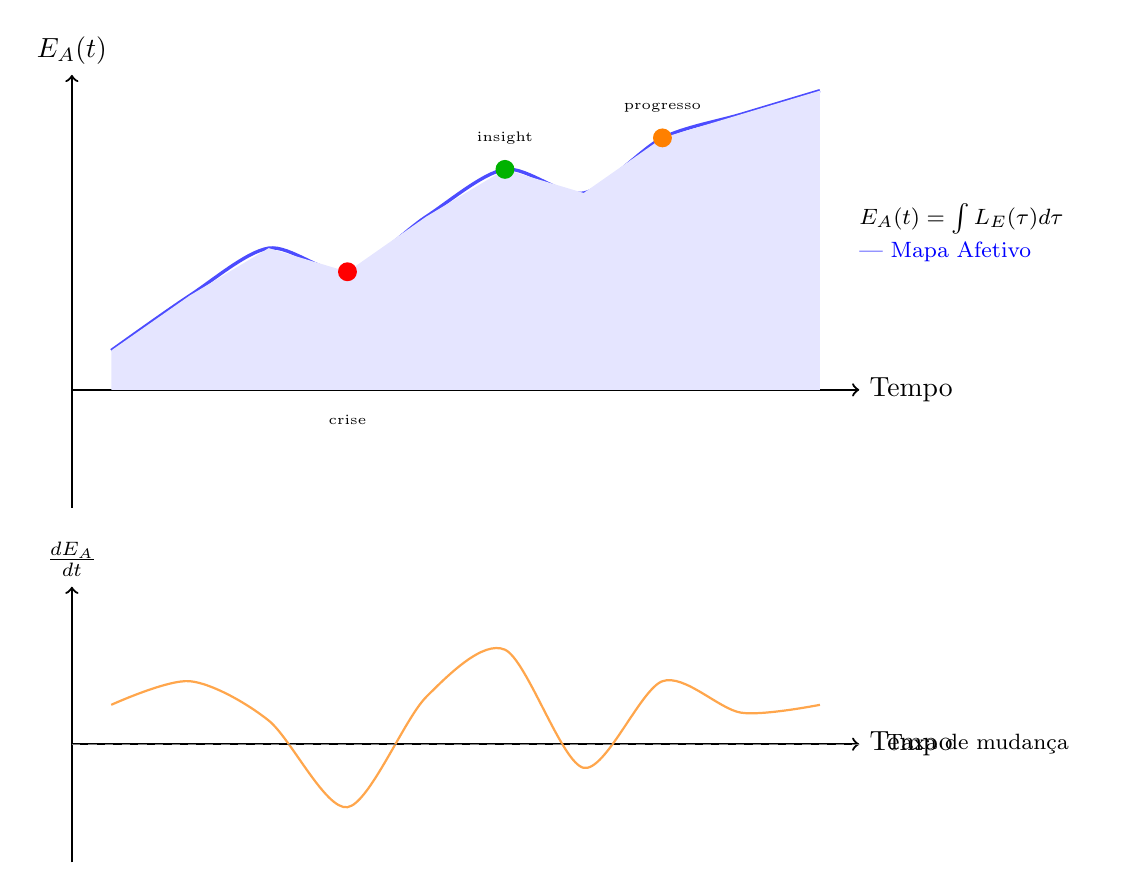
\begin{tikzpicture}[scale=1]
    % Gráfico do Mapa Afetivo
    \begin{scope}
        % Eixos
        \draw[thick, ->] (0,0) -- (10,0) node[right] {Tempo};
        \draw[thick, ->] (0,-1.5) -- (0,4) node[above] {$E_A(t)$};

        % Curva do mapa afetivo (integral)
        \draw[very thick, blue!70, smooth] plot coordinates {
            (0.5,0.5) (1.5,1.2) (2.5,1.8) (3.5,1.5) (4.5,2.2) (5.5,2.8) (6.5,2.5) (7.5,3.2) (8.5,3.5) (9.5,3.8)
        };

        % Área sob a curva (representando acumulação)
        \fill[blue!10] (0.5,0) -- plot coordinates {
            (0.5,0.5) (1.5,1.2) (2.5,1.8) (3.5,1.5) (4.5,2.2) (5.5,2.8) (6.5,2.5) (7.5,3.2) (8.5,3.5) (9.5,3.8)
        } -- (9.5,0) -- cycle;

        % Pontos de intervenção
        \fill[red] (3.5,1.5) circle (0.12);
        \fill[green!70!black] (5.5,2.8) circle (0.12);
        \fill[orange] (7.5,3.2) circle (0.12);

        % Labels
        \node[font=\tiny, below] at (3.5,-0.2) {crise};
        \node[font=\tiny, above] at (5.5,3) {insight};
        \node[font=\tiny, above] at (7.5,3.4) {progresso};

        % Legenda
        \node[font=\footnotesize, text width=3cm, align=left] at (11.5,2) {
            $E_A(t) = \int L_E(\tau)d\tau$\\[0.3em]
            \textcolor{blue}{--- Mapa Afetivo}
        };
    \end{scope}

    % Gráfico da derivada (abaixo)
    \begin{scope}[shift={(0,-4.5)}]
        \draw[thick, ->] (0,0) -- (10,0) node[right] {Tempo};
        \draw[thick, ->] (0,-1.5) -- (0,2) node[above] {$\frac{dE_A}{dt}$};

        % Curva da derivada
        \draw[thick, orange!70, smooth] plot coordinates {
            (0.5,0.5) (1.5,0.8) (2.5,0.3) (3.5,-0.8) (4.5,0.6) (5.5,1.2) (6.5,-0.3) (7.5,0.8) (8.5,0.4) (9.5,0.5)
        };

        % Linha zero
        \draw[dashed, gray] (0,0) -- (10,0);

        \node[font=\footnotesize] at (11.5,0) {Taxa de mudança};
    \end{scope}
\end{tikzpicture}
\end{center}

\begin{sintese}[title=Síntese Final da Seção 4]
O estado emocional é acumulado ao longo do tempo, formando um mapa afetivo que pode ser traçado e compreendido através da análise longitudinal da linguagem. Ao integrar as expressões emocionais, revelam-se padrões e oscilações internas que, muitas vezes, permanecem ocultos à consciência imediata. Este mapeamento permite ao terapeuta e ao paciente identificar trajetórias emocionais, promover insights profundos e intervir de forma precisa no processo terapêutico.

Inspirados por Lacan, reconhecemos que a linguagem estrutura o inconsciente, e através dela podemos acessar os significantes que moldam o self. Dennett e Searle nos lembram da importância da narrativa contínua e da intencionalidade dos estados mentais na construção da consciência. O mapa afetivo construído pela linguagem ao longo do tempo não é apenas uma ferramenta diagnóstica, mas um guia para a construção do self autêntico e para a promoção da autonomia do ser.
\end{sintese}

\nextpage
